\section{Azerbaijan Grand Prix}

\subsection{Circuit Analysis}

\textbf{Circuit Name:} Baku City Circuit (Baku, Azerbaijan) \\
\textbf{Length:} 6.003 km - \textbf{Laps:} 51 - \textbf{Total Distance:} 306.049 km

\begin{figure}[H]
    \centering
    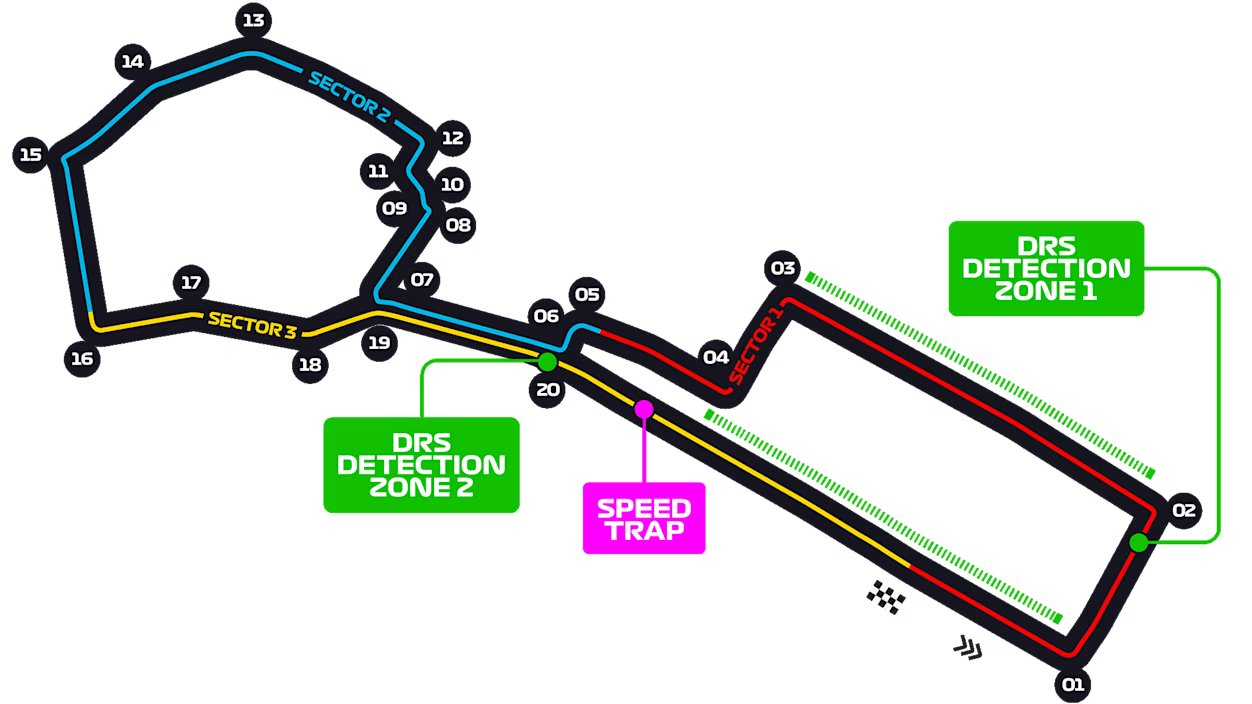
\includegraphics[width=0.75\linewidth]{images/17.Azerbaijan_Circuit.jpg}
\end{figure}

\begin{itemize}
    \item \textbf{Lap Record} : 1:40.203 (2023, Charles Leclerc – Ferrari).

    \item \textbf{Number of Corners \& Key Features} : 20 turns (8 right, 12 left). \\
    Longest straight (2.2 km) with DRS, mixed with narrow old town section (Turns 8–12). \\
    Demands low downforce for speed yet stability for traction/braking in tight corners.

    \item \textbf{Braking Zones \& Traction} : Major braking at Turn 1 (end of main straight), Turn 3, and Turn 15. \\
    Rear traction out of low-speed corners is critical, especially final corner before the main straight.

    \item \textbf{DRS \& Overtaking} : Two main DRS zones (main straight and between Turns 2–3). \\
    Prime overtaking into Turn 1, opportunistic moves possible at Turn 3.

    \item \textbf{Tyre Degradation \& Strategy} : Surface relatively smooth → low wear, but rear degradation can spike due to traction zones. \\
    Safety Car probability is high, influencing flexible tyre strategies.

    \item \textbf{Weather \& Environment} : Usually hot and dry. Winds from the Caspian Sea affect top speed and braking points.
\end{itemize}

\textbf{Strategic Summary :} Baku mixes extreme top-speed demand with technical old-town precision. Teams must balance low-drag setups with enough grip for traction zones. Strategy must stay flexible due to frequent Safety Cars.

\subsection{Race Analysis}

\textbf{Date:} 15 September 2024 — 15:00 local time

\begin{itemize}
    \item \textbf{Qualifying Summary} : \textbf{Pole Position:} Charles Leclerc (Ferrari) – 1:41.365. \\
    Grid: Piastri 2nd, Sainz 3rd, Pérez 4th. \\
    Norris only P15 after poor session, Hamilton penalised to pitlane start.

    \item \textbf{Race Summary} : \textbf{Winner:} Oscar Piastri (McLaren). \\
    \textbf{Podium:} 1. Piastri - 2. Leclerc - 3. Russell. \\
    \textbf{Notable incidents:} Sainz-Pérez collision while fighting for podium on the next-to-last lap, (Virtual Safety Car deployed, both cars retired). \\
    Piastri overtook Leclerc on lap 20 with DRS on main straight and never looked back. \\
    Norris recovered to P4 with fastest lap. Williams scored double points with Albon (P7) and rookie Colapinto (P8).

    \item \textbf{Strategies} : 
    - Tyre degradation low : mix of one- and two-stop strategies. \\
    - Piastri: Medium–Hard (lap 14) — early stop + undercut worked perfectly (form 6s to 1s behind Leclerc). \\
    - Leclerc: Medium–Hard (lap 15) — track position lost to Piastri’s undercut, tyres faded late. \\
    - Norris: aggressive two-stop (Medium–Hard–Soft) → fastest lap, strong comeback. \\
    - Red Bull struggled: Verstappen conservative Medium–Hard, lacked pace.

    \item \textbf{Performance Trends} : \textbf{McLaren} strong in straights and tyre life — Piastri flawless, Norris rapid in traffic. \\
    \textbf{Ferrari} fast over one lap but weaker in long runs, Leclerc fading late. \\
    \textbf{Red Bull} lacked stability, Verstappen complained of brakes and grip. \\
    \textbf{Williams} breakthrough with Albon P7 and Colapinto P8. \\
    \textbf{Mercedes} consistent, Russell podium with opportunism.

    \item \textbf{Championship Impact} : \textbf{Drivers:} Verstappen 313, Norris 254, Leclerc 235. \\
    \textbf{Constructors:} McLaren 476 (+1), Red Bull 456 (-1), Ferrari 425, Mercedes 309.
\end{itemize}

\textbf{Key Takeaway :} Piastri’s precision and tyre management secured McLaren’s rise to the top of the Constructors’ standings, while Ferrari maximised Leclerc’s pole pace but fell short in race management.

\subsection{Link \& Takeaway}

\begin{itemize}
    \item Baku’s ultra-long straights amplified McLaren’s low-drag efficiency, enabling Piastri to overtake and control pace. 
    \item Ferrari’s one-lap advantage from higher downforce backfired in tyre life and straight-line speed. 
    \item Red Bull’s balance issues highlighted difficulty in braking and traction, critical weaknesses at Baku.
    \item Williams capitalised on Baku’s traction demands and long straights to deliver double points. 
    \item Ultimately, McLaren’s ability to blend straight-line speed with flexible tyre strategy proved decisive, shifting momentum in both championships.
\end{itemize}
